\begin{appendices}
	\section*{Imágenes de algunas anomalías en la carretera}
		\begin{figure}[htb]
			  \centering
			  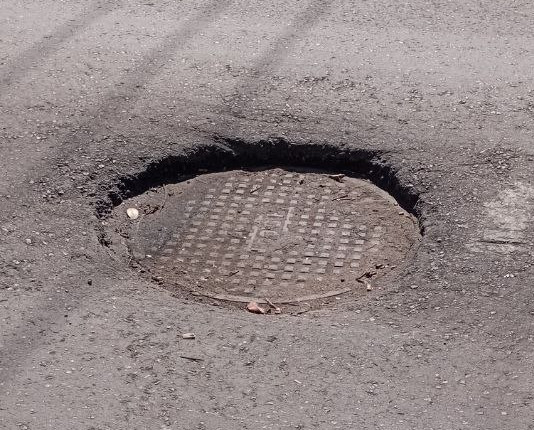
\includegraphics[scale = 0.4]{Graphics/pothole_3.jpg}
			  \caption{Boca de alcantarilla hundida en el pavimento}
			  \label{fig:13}
		\end{figure}

		\begin{figure}[htb]
			  \centering
			  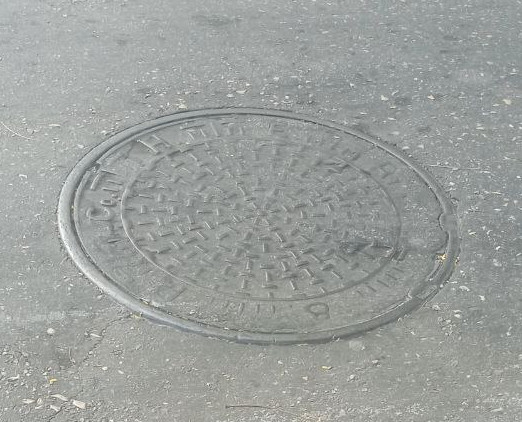
\includegraphics[scale = 0.4]{Graphics/pothole_9.jpg}
			  \caption{Boca de alcantarilla}
			  \label{fig:14}
		\end{figure}
		\newpage

		\begin{figure}[htb]
			\centering
			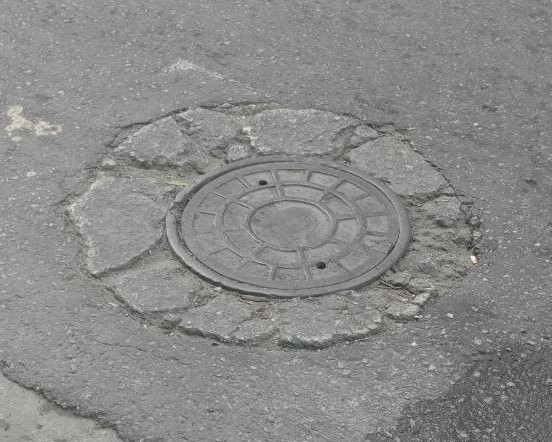
\includegraphics[scale = 0.3]{Graphics/pothole_4.jpg}
			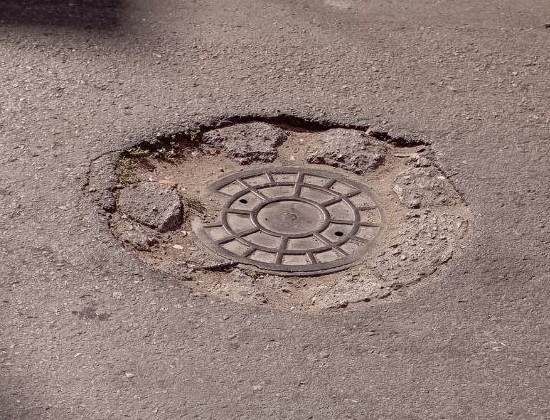
\includegraphics[scale = 0.3]{Graphics/pothole_5.jpg}
			\caption{tapas de alcantarilla con características anormales}
			\label{fig:15}
		\end{figure}
		\newpage

		\begin{figure}[htb]
			\centering
			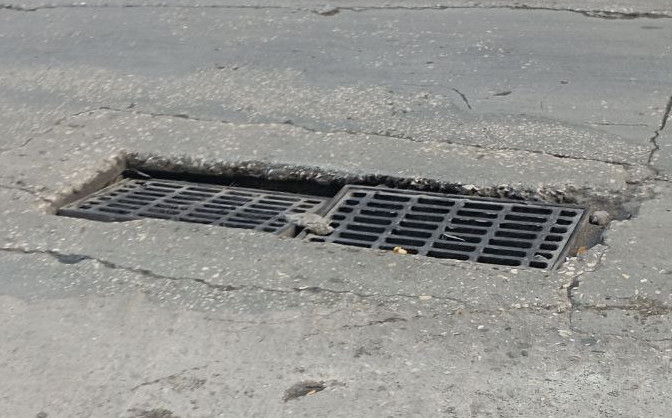
\includegraphics[scale = 0.3]{Graphics/pothole_10.jpg}
			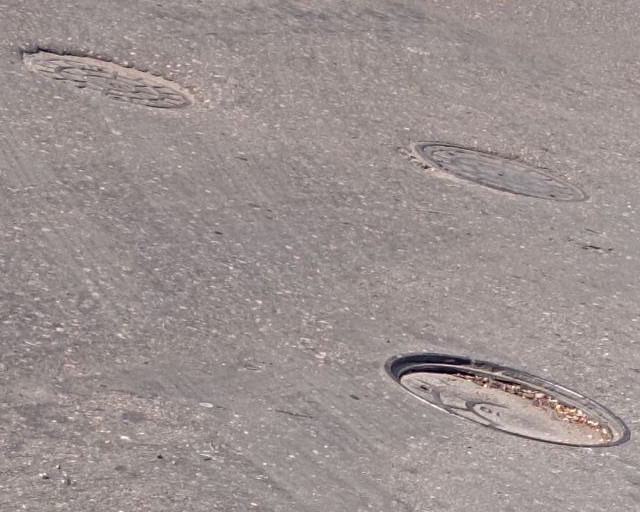
\includegraphics[scale = 0.3]{Graphics/pothole_11.jpg}
			\caption{Otros objetos en la vía con características anormales}
			\label{fig:16}
		\end{figure}

		\begin{figure}[htb]
			\centering
			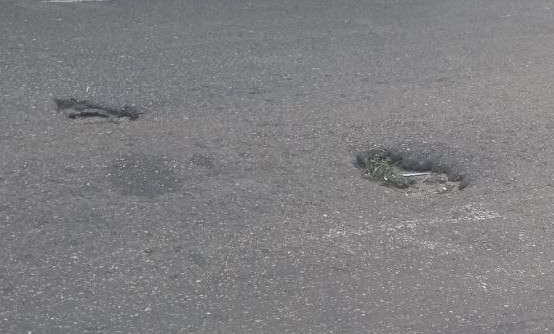
\includegraphics[scale = 0.3]{Graphics/pothole_7.jpg}
			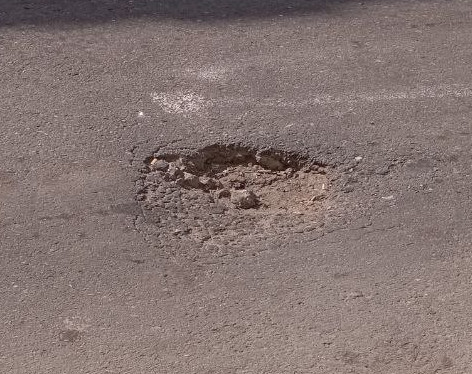
\includegraphics[scale = 0.3]{Graphics/pothole_8.jpg}
			\caption{Algunos baches de algunas de las rutas seleccionadas}
			\label{fig:17}
		\end{figure}

		\newpage
		\begin{figure}[htb]
			\centering
			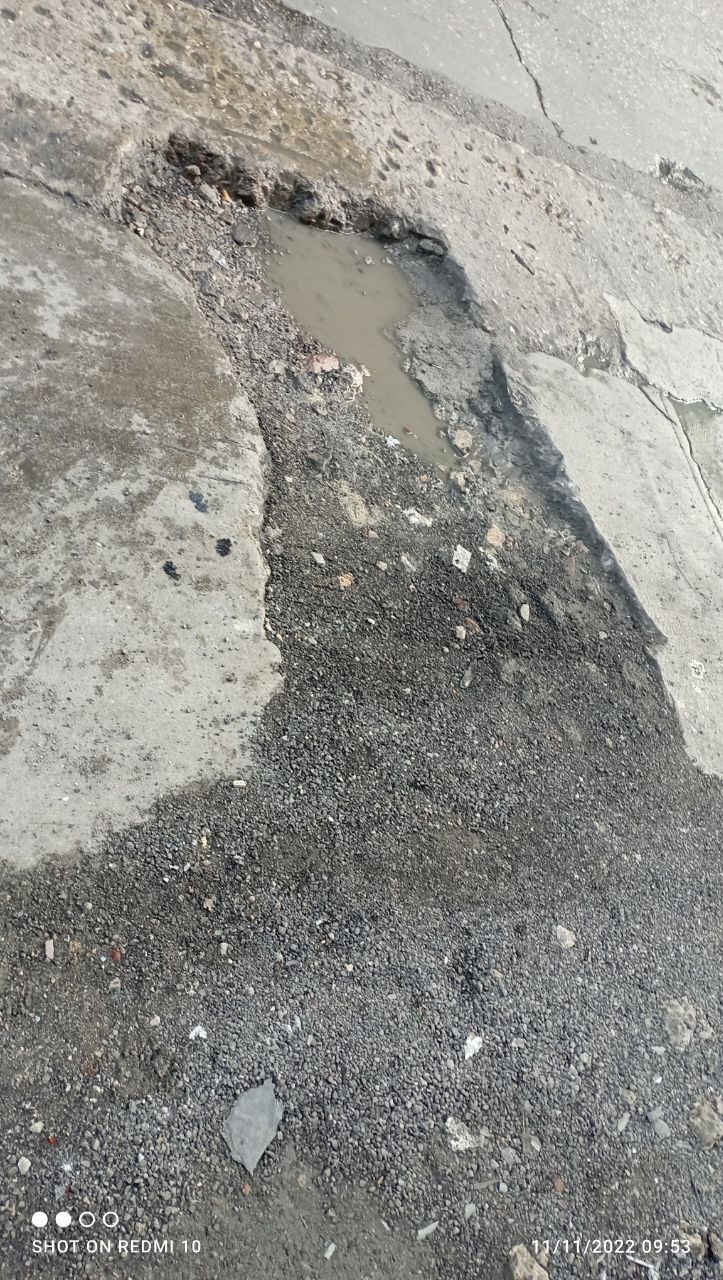
\includegraphics[scale = 0.3]{Graphics/pothole_1.jpg}
			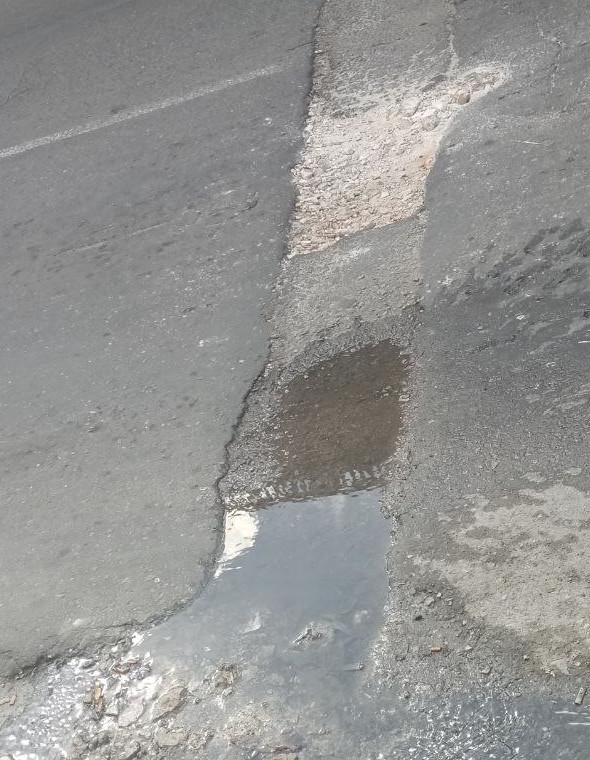
\includegraphics[scale = 0.3]{Graphics/pothole_2.jpg}
			\caption{Más baches de algunas de las rutas seleccionadas}
			\label{fig:18}
		\end{figure}
		\newpage

	\section*{Tablas con los hiperparámetros que se probaron para los métodos no-supervisados}
		\begin{figure}[htb]
			\centering
			\begin{tabular}{ll}
				\toprule
				                                          eps &                                  min\_samples \\
				\midrule
				  0.05, 0.1, ..., 0.95, 0.99 &  15, 20, ..., 60, 65 \\
				\bottomrule
			\end{tabular}
			\caption{Hyperparámetros con los que se probó \textbf{DBSCAN}}
			\label{table:4}
		\end{figure}
		
		\begin{figure}[htb]
			\centering
			\begin{tabular}{ll}
				\toprule
				                                            gamma &                                                 nu \\
				\midrule
				  scale, 0.00001, 0.0001, 0.001, 0.01, 0.1, 1, 10 &  0.05, 0.1, ..., 0.95, 0.99 \\
				\bottomrule
			\end{tabular}
			\caption{Hyperparámetros con los que se probó \textbf{One Class SVM}}
			\label{table:5}
		\end{figure}
		
		\begin{figure}[htb]
			\centering
			\begin{tabular}{lll}
				\toprule
				 cluster\_method &                                      metric &                                        min\_samples \\
				\midrule
				     xi, dbscan &  minkowski, euclidean, canberra, braycurtis &  5, 10, ..., 60, 65 \\
				\bottomrule
			\end{tabular}
			\caption{Hyperparámetros con los que se probó \textbf{OPTICS}}
			\label{table:6}
		\end{figure}

	\section*{Tablas con los hiperparámetros que se probaron para los métodos supervisados}
		\begin{figure}[ht!]
			\centering
			\begin{tabular}{llll}
				\toprule
					   n\_neighbors &            weights &                  algorithm &       leaf\_size \\
				\midrule
				 3, 5, 7, 9, 11 &  uniform, distance &  brute, kd\_tree, ball\_tree &  20, 30, 40, 50 \\
				\bottomrule
			\end{tabular}
			\caption{Hiperparámetros \textbf{KNN}}
			\label{table:7}
		\end{figure}

		\begin{figure}[ht!]
			\centering
			\begin{tabular}{llll}
				\toprule
						criterion &        splitter &           max\_depth &      max\_features \\
				\midrule
				  entropy, gini &  best, random &  3, 4, 5, 6, None &  sqrt, log2, None \\
				\bottomrule
			\end{tabular}
			\caption{Hiperparámetros \emph{Decision Tree}}
			\label{table:8}
		\end{figure}
		
		\begin{figure}[ht!]
			\centering
			\begin{tabular}{llll}
				\toprule
					 n\_estimators &        criterion &          max\_depth &  max\_features \\
				\midrule
				  100, 120, 180 &  entropy, gini &  10,  13, 16, 20 &  log2, sqrt \\
				\bottomrule
			\end{tabular}
			\caption{Hiperparámetros \emph{Randon Forest}}
			\label{table:9}
		\end{figure}

		\begin{figure}[ht!]
			\centering
			\begin{tabular}{lllll}
				\toprule
				 penalty &                       tol &                   C &         solver &        max\_iter \\
				\midrule
					l2 &  1e-3, 1e-4, 1e-5, 1e-6 &  1, 10, 100, 1000 &  lbfgs, saga &  100, 500, 1000 \\
				\bottomrule
			\end{tabular}
			\caption{Hiperparámetros regresión logística}
			\label{table:10}
		\end{figure}
		\newpage

		\begin{figure}[ht!]
			\centering
			\begin{tabular}{llll}
				\toprule
					  C & kernel &          gamma &  probability \\
				\midrule
				  100 &  rbf &  0.01, 0.001 &         True \\
				\bottomrule
			\end{tabular}
			\caption{Hiperparámetros \textbf{SVM}}
			\label{table:11}
		\end{figure}
		\newpage

	\section*{Tablas de resultados}
		\begin{figure}[htb]
			\centering
			\begin{tabular}{ll}
				\toprule
					  outliers\_method &                                z\_thresh \\
					 feature\_selector &                       forward\_selection \\
				features\_selected\_set & {Y Accel, MeanDevGyroX, MedianDevGyroX} \\
								Model &                                     KNN \\
						f1\_score &                                   0.125 \\
					   precision &                                     0.1 \\
						  recall &                                0.166667 \\
						accuracy &                                0.517241 \\
				\bottomrule
			\end{tabular}
			\newline
			\newline

			\begin{tabular}{ll}
				\toprule
				Hyperparams &   Value \\
				\midrule
				  algorithm &   brute \\
				n\_neighbors &       3 \\
					weights & uniform \\
				\bottomrule
			\end{tabular}
			\caption{Mejor resultado obtenido con \textbf{Z-Thresh} y \textbf{KNN}}
			\label{table:14}
		\end{figure}

		\begin{figure}[htb]
			\centering
			\begin{tabular}{ll}
				\toprule
					  outliers\_method &                                       z\_diff \\
					 feature\_selector &                            forward\_selection \\
				features\_selected\_set & {MeanDevGyroX, MedianDevGyroY, MeanDevGyroZ} \\
								Model &                                          KNN \\
						F1\_score &                                     0.266667 \\
					   Precision &                                     0.285714 \\
						  Recall &                                         0.25 \\
						Accuracy &                                          0.6 \\
				\bottomrule
			\end{tabular}
			\newline
			\newline

			\begin{tabular}{ll}
				\toprule
				Hyperparams &    Value \\
				\midrule
				  algorithm &  kd\_tree \\
				  leaf\_size &       50 \\
				n\_neighbors &        3 \\
					weights & distance \\
				\bottomrule
			\end{tabular}
			\caption{Mejor resultado obtenido con \textbf{Z-Diff} y \textbf{KNN}}
			\label{table:14}
		\end{figure}

		\begin{figure}[htb]
			\centering
			\begin{tabular}{ll}
				\toprule
					  Outliers\_method &                                   dbscan \\
					 Feature\_selector &                        forward\_selection \\
				Features\_selected\_set & \{X / Z, MedianDevAccelY, MedianDevGyroZ\} \\
								Model &                                      KNN \\
						F1\_score &                                 0.521739 \\
					   Precision &                                      0.6 \\
						  Recall &                                 0.461538 \\
						Accuracy &                                 0.731707 \\
				\bottomrule
			\end{tabular}
			\newline
			\newline

			\begin{tabular}{ll}
				\toprule
				Hyperparams &     Value \\
				\midrule
				  algorithm & ball\_tree \\
				  leaf\_size &        30 \\
				n\_neighbors &         3 \\
					weights &  distance \\
				\bottomrule
			\end{tabular}
			\caption{Mejor resultado obtenido con \textbf{DBSCAN} y \textbf{KNN}}
			\label{table:12}
		\end{figure}

		\begin{figure}[htb]
			\centering
			\begin{tabular}{ll}
				\toprule
					  outliers\_method &                                  ocsvm \\
					 feature\_selector &                      forward\_selection \\
				features\_selected\_set & \{X Gyro, MeanDevAccelY, MeanDevAccelZ\} \\
								Model &                                    KNN \\
						F1\_score &                               0.327273 \\
					   Precision &                               0.409091 \\
						  Recall &                               0.272727 \\
						Accuracy &                               0.723881 \\
				\bottomrule
			\end{tabular}
			\newline
			\newline

			\begin{tabular}{ll}
				\toprule
				Hyperparams &     Value \\
				\midrule
				  algorithm & ball\_tree \\
				  leaf\_size &        30 \\
				n\_neighbors &         3 \\
					weights &  distance \\
				\bottomrule
			\end{tabular}
			\caption{Mejor resultado obtenido con \textbf{One Class SVM} y \textbf{KNN}}
			\label{table:13}
		\end{figure}

		\begin{figure}[htb]
			\centering
			\begin{tabular}{ll}
				\toprule
					  outliers\_method &                                           z\_thresh \\
					 feature\_selector &                              recursive\_elimination \\
					 features\_selected\_set & \{Y Gyro, X / Z, MaxZratio, MinZratio, SpeedvsZ, MeanDevGyroX\} \\
								Model &                                      Decision Tree \\
						F1\_score &                                           0.363636 \\
					   Precision &                                               0.25 \\
						  Recall &                                           0.666667 \\
						Accuracy &                                           0.517241 \\
				\bottomrule
			\end{tabular}
			\newline
			\newline

			\begin{tabular}{ll}
			\toprule
			 Hyperparams &   Value \\
			\midrule
			   criterion & entropy \\
			   max\_depth &    None \\
			max\_features &    log2 \\
				splitter &    best \\
			\bottomrule
			\end{tabular}
			\caption{Mejor resultado obtenido con \textbf{Z-Thresh} y \emph{Decision Tree}}
			\label{table:14}
		\end{figure}

		\begin{figure}[htb]
			\centering
			\begin{tabular}{ll}
				\toprule
					  outliers\_method &                                    z\_diff \\
					 feature\_selector &                         forward\_selection \\
				features\_selected\_set & \{MinZratio, MedianDevGyroY, MeanDevGyroZ\} \\
								Model &                             Decision Tree \\
						F1\_score &                                  0.333333 \\
					   Precision &                                  0.357143 \\
						  Recall &                                    0.3125 \\
						Accuracy &                                  0.636364 \\
				\bottomrule
			\end{tabular}
			\newline
			\newline

			\begin{tabular}{ll}
				\toprule
				 Hyperparams &   Value \\
				\midrule
				   criterion & entropy \\
				   max\_depth &    None \\
				max\_features &    None \\
					splitter &    best \\
				\bottomrule
			\end{tabular}
			\caption{Mejor resultado obtenido con \textbf{Z-Diff} y \emph{Decision Tree}}
			\label{table:14}
		\end{figure}

		\begin{figure}[htb]
			\centering
			\begin{tabular}{ll}
				\toprule
					  outliers\_method &                               dbscan \\
					 feature\_selector &                recursive\_elimination \\
				features\_selected\_set & \{X / Z, MeanDevAccelY, MeanDevGyroY\} \\
								Model &                        Decision Tree \\
						F1\_score &                             0.551724 \\
					   Precision &                                  0.5 \\
						  Recall &                             0.615385 \\
						Accuracy &                             0.682927 \\
				\bottomrule
			\end{tabular}
			\newline
			\newline

			\begin{tabular}{ll}
				\toprule
				 Hyperparams &   Value \\
				\midrule
				   criterion & entropy \\
				   max\_depth &    None \\
				max\_features &    None \\
					splitter &    best \\
				\bottomrule
			\end{tabular}
			\caption{Mejor resultado obtenido con \textbf{DBSCAN} y \emph{Decision Tree}}
			\label{table:15}
		\end{figure}

		\begin{figure}[htb]
			\centering
			\begin{tabular}{ll}
				\toprule
					  outliers\_method &                                              ocsvm \\
					 feature\_selector &                              recursive\_elimination \\
				features\_selected\_set & \{Y Accel, X Gyro, Y Gyro, X / Z, MinZratio, SpeedvsZ \\
									{} & MeanDevAccelX, MeanDevAccelY, MeanDevGyroX\} \\
								Model &                                      Decision Tree \\
						F1\_score &                                           0.492308 \\
					   Precision &                                                0.5 \\
						  Recall &                                           0.484848 \\
						Accuracy &                                           0.753731 \\
				\bottomrule
			\end{tabular}
			\newline
			\newline

			\begin{tabular}{ll}
				\toprule
				 Hyperparams &   Value \\
				\midrule
				   criterion & entropy \\
				   max\_depth &    None \\
				max\_features &    None \\
					splitter &    best \\
				\bottomrule
			\end{tabular}
			\caption{Mejor resultado obtenido con \textbf{One Class SVM} y \emph{Decision Tree}}
			\label{table:16}
		\end{figure}

		\begin{figure}[htb]
			\centering
			\begin{tabular}{ll}
				\toprule
					  outliers\_method &                                   z\_thresh \\
					 feature\_selector &                          forward\_selection \\
				features\_selected\_set & \{Y Accel, MedianDevAccelX, MedianDevGyroX\} \\
								Model &                                        SVM \\
						F1\_score &                                       0.25 \\
					   Precision &                                        0.2 \\
						  Recall &                                   0.333333 \\
						Accuracy &                                   0.586207 \\
				\bottomrule
			\end{tabular}
			\newline
			\newline

			\begin{tabular}{ll}
				\toprule
				Hyperparams & Value \\
				\midrule
						  C &  1000 \\
					  gamma &  0.01 \\
					 kernel &   rbf \\
				probability &  true \\
				\bottomrule
			\end{tabular}
			\caption{Mejor resultado obtenido con \textbf{Z-Thresh} y \textbf{SVM}}
			\label{table:17}
		\end{figure}

		\begin{figure}[htb]
			\centering
			\begin{tabular}{ll}
				\toprule
					  outliers\_method &                            z\_diff \\
					 feature\_selector &                 forward\_selection \\
				features\_selected\_set & \{Z Accel, SpeedvsZ, MeanDevGyroZ\} \\
								Model &                               SVM \\
						F1\_score &                          0.222222 \\
					   Precision &                          0.272727 \\
						  Recall &                            0.1875 \\
						Accuracy &                          0.618182 \\
				\bottomrule
			\end{tabular}
			\newline
			\newline

			\begin{tabular}{ll}
				\toprule
				Hyperparams & Value \\
				\midrule
						  C &  1000 \\
					  gamma &  0.01 \\
					 kernel &   rbf \\
				probability &  true \\
				\bottomrule
			\end{tabular}
			\caption{Mejor resultado obtenido con \textbf{Z-Diff} y \textbf{SVM}}
			\label{table:18}
		\end{figure}

		\begin{figure}[htb]
			\centering
			\begin{tabular}{ll}
				\toprule
					  outliers\_method &                                    dbscan \\
					 feature\_selector &                         forward\_selection \\
				features\_selected\_set & \{SpeedvsZ, MedianDevAccelY, MeanDevGyroY\} \\
								Model &                                       SVM \\
						F1\_score &                                       0.5 \\
					   Precision &                                  0.545455 \\
						  Recall &                                  0.461538 \\
						Accuracy &                                  0.707317 \\
				\bottomrule
			\end{tabular}
			\newline
			\newline

			\begin{tabular}{ll}
				\toprule
				Hyperparams & Value \\
				\midrule
						  C &    10 \\
					  gamma &   0.1 \\
					 kernel &   rbf \\
				probability &  true \\
				\bottomrule
			\end{tabular}
			\caption{Mejor resultado obtenido con \textbf{DBSCAN} y \textbf{SVM}}
			\label{table:19}
		\end{figure}

		\begin{figure}[htb]
			\centering
			\begin{tabular}{ll}
				\toprule
					  outliers\_method &                                ocsvm \\
					 feature\_selector &                    forward\_selection \\
				features\_selected\_set & \{X / Z, MeanDevAccelZ, MeanDevGyroX\} \\
								Model &                                  SVM \\
						F1\_score &                             0.285714 \\
					   Precision &                             0.347826 \\
						  Recall &                             0.242424 \\
						Accuracy &                             0.701493 \\
				\bottomrule
			\end{tabular}
			\newline
			\newline

			\begin{tabular}{ll}
				\toprule
				Hyperparams & Value \\
				\midrule
						  C &  1000 \\
					  gamma &  0.01 \\
					 kernel &   rbf \\
				probability &  true \\
				\bottomrule
			\end{tabular}
			\caption{Mejor resultado obtenido con \textbf{One Class SVM} y \textbf{SVM}}
			\label{table:19}
		\end{figure}

		\begin{figure}[htb]
			\centering
			\begin{tabular}{ll}
				\toprule
					  outliers\_method &                                           z\_thresh \\
					 feature\_selector &                                  forward\_selection \\
				features\_selected\_set & \{Z Accel, MinZratio, MedianDevAccelX, MeanDevAccelY \\
									{} &  MeanDevAccelZ, MeanDevGyroX, MedianDevGyroX, \\
									{} &  MeanDevGyroY, MedianDevGyroY\}\\
								Model &                                     Log Regression \\
						F1\_score &                                           0.266667 \\
					   Precision &                                           0.333333 \\
						  Recall &                                           0.222222 \\
						Accuracy &                                            0.62069 \\
				\bottomrule
			\end{tabular}
			\newline
			\newline

			\begin{tabular}{ll}
				\toprule
				Hyperparams &   Value \\
				\midrule
						  C &     100 \\
				   max\_iter &     500 \\
					penalty &      l2 \\
					 solver &    saga \\
						tol &  0.0001 \\
				\bottomrule
			\end{tabular}
			\caption{Mejor resultado obtenido con \textbf{Z-Thresh} y \textbf{Regresión Logística}}
			\label{table:20}
		\end{figure}

		\begin{figure}[htb]
			\centering
			\begin{tabular}{ll}
				\toprule
					  outliers\_method &                            z\_diff \\
					 feature\_selector &                 forward\_selection \\
				features\_selected\_set & \{Y Accel, X / Z, MedianDevAccelY\} \\
								Model &                    Log Regression \\
						F1\_score &                          0.363636 \\
					   Precision &                               0.4 \\
						  Recall &                          0.333333 \\
						Accuracy &                          0.618182 \\
				\bottomrule
			\end{tabular}
			\newline
			\newline

			\begin{tabular}{ll}
				\toprule
				Hyperparams &    Value \\
				\midrule
						  C &      100 \\
				   max\_iter &      500 \\
					penalty &       l2 \\
					 solver &    lbfgs \\
						tol &  0.00001 \\
				\bottomrule
			\end{tabular}
			\caption{Mejor resultado obtenido con \textbf{Z-Diff} y \textbf{Regresión Logística}}
			\label{table:21}
		\end{figure}

		\begin{figure}[htb]
			\centering
			\begin{tabular}{ll}
				\toprule
					  outliers\_method &                                   dbscan \\
					 feature\_selector &                        forward\_selection \\
				features\_selected\_set & \{X / Z, MedianDevAccelY, MedianDevGyroZ\} \\
								Model &                           Log Regression \\
						F1\_score &                                 0.210526 \\
					   Precision &                                 0.222222 \\
						  Recall &                                      0.2 \\
						Accuracy &                                 0.634146 \\
				\bottomrule
			\end{tabular}
			\newline
			\newline

			\begin{tabular}{ll}
				\toprule
				Hyperparams &     Value \\
				\midrule
						  C &       100 \\
				   max\_iter &       500 \\
					penalty &        l2 \\
					 solver &     lbfgs \\
						tol &  0.000001 \\
				\bottomrule
			\end{tabular}
			\caption{Mejor resultado obtenido con \textbf{DBSCAN} y \textbf{Regresión Logística}}
			\label{table:22}
		\end{figure}

		\begin{figure}[htb]
			\centering
			\begin{tabular}{ll}
				\toprule
					  outliers\_method &                                          ocsvm \\
					 feature\_selector &                              forward\_selection \\
				features\_selected\_set & \{MedianDevAccelY, MeanDevAccelZ, MeanDevGyroZ\} \\
								Model &                                 Log Regression \\
						F1\_score &                                        0.27907 \\
					   Precision &                                            0.6 \\
						  Recall &                                       0.181818 \\
						Accuracy &                                       0.768657 \\
				\bottomrule
			\end{tabular}
			\newline
			\newline

			\begin{tabular}{ll}
				\toprule
				Hyperparams &  Value \\
				\midrule
						  C &    100 \\
				   max\_iter &    100 \\
					penalty &     l2 \\
					 solver &   saga \\
						tol &  0.001 \\
				\bottomrule
			\end{tabular}
			\caption{Mejor resultado obtenido con \textbf{One Class SVM} y \textbf{Regresión Logística}}
			\label{table:23}
		\end{figure}

		\begin{figure}[htb]
			\centering
			\begin{tabular}{ll}
				\toprule
					  outliers\_method &                                           z\_thresh \\
					 feature\_selector &                                 backward\_selection \\
				features\_selected\_set &  \{Y Accel, Z Accel, X Gyro, Y Gyro, SpeedvsZ, MeanDevAccelZ,\\
										& MeanDevGyroX, MeanDevGyroY, MedianDevGyroZ\}\\
								model &                                      Random Forest \\
							 F1\_score &                                           0.428571 \\
							Precision &                                              0.375 \\
							   Recall &                                                0.5 \\
							 Accuracy &                                           0.724138 \\
				\bottomrule
			\end{tabular}
			\newline
			\newline
			
			\begin{tabular}{ll}
				\toprule
				 Hyperparams & Value \\
				\midrule
				   criterion &  gini \\
				   max\_depth &     6 \\
				max\_features &  sqrt \\
				n\_estimators &   100 \\
				\bottomrule
			\end{tabular}
			\caption{Mejor resultado obtenido con \textbf{Z-Thresh} y \textbf{Random Forest}}
			\label{table:24}
		\end{figure}
		
		\begin{figure}[htb]
			\centering

			\begin{tabular}{ll}
				\toprule
					  outliers\_method &                                             z\_diff \\
					 feature\_selector &                                 backward\_selection \\
				features\_selected\_set & \{Z Accel, Y Gyro, MinZratio, SpeedvsZ, MeanDevAccelZ, \\
                						& MeanDevGyroX, MedianDevGyroX, MeanDevGyroY,\\ 
										& MedianDevGyroY\} \\
								model &                                      Random Forest \\
							 F1\_score &                                           0.434783 \\
							Precision &                                           0.714286 \\
							   Recall &                                             0.3125 \\
							 Accuracy &                                           0.763636 \\
				\bottomrule
			\end{tabular}
			\newline
			\newline

			\begin{tabular}{ll}
				\toprule
				 Hyperparams & Value \\
				\midrule
				   criterion &  gini \\
				   max\_depth &    20 \\
				max\_features &  sqrt \\
				n\_estimators &   120 \\
				\bottomrule
			\end{tabular}
			\caption{Mejor resultado obtenido con \textbf{Z-Diff} y \textbf{Random Forest}}
			\label{table:25}

		\end{figure}

		\begin{figure}[htb]
			\centering
			\begin{tabular}{ll}
				\toprule
					  outliers\_method &                                             dbscan \\
					 feature\_selector &                              recursive\_elimination \\
				features\_selected\_set & \{X Accel, Y Accel, Y Gyro, Z Gyro, X / Z, SpeedvsZ\}\\
								model &                                      Random Forest \\
							 F1\_score &                                           0.545455 \\
							Precision &                                           0.666667 \\
							   Recall &                                           0.461538 \\
							 Accuracy &                                           0.756098 \\
				\bottomrule
			\end{tabular}
			\newline
			\newline

			\begin{tabular}{ll}
				\toprule
				 Hyperparams & Value \\
				\midrule
				   criterion &  gini \\
				   max\_depth &    10 \\
				max\_features &  log2 \\
				n\_estimators &   180 \\
				\bottomrule
			\end{tabular}
			\caption{Mejor resultado obtenido con \textbf{DBSCAN} y \textbf{Random Forest}}
			\label{table:26}

		\end{figure}

		\begin{figure}[htb]
			\centering
			\begin{tabular}{ll}
				\toprule
					  outliers\_method &                                              ocsvm \\
					 feature\_selector &                                  forward\_selection \\
				features\_selected\_set & \{X Gyro, Y Gyro, Z Gyro, X / Z, MeanDevAccelY\\
										&	MeanDevAccelZ, MedianDevGyroY, MeanDevGyroZ,\\ 
										& MedianDevGyroZ\} \\
								model &                                      Random Forest \\
							 F1\_score &                                           0.292683 \\
							Precision &                                               0.75 \\
							   Recall &                                           0.181818 \\
							 Accuracy &                                           0.783582 \\
				\bottomrule
			\end{tabular}
			\newline
			\newline
			
			\begin{tabular}{ll}
				\toprule
				 Hyperparams & Value \\
				\midrule
				   criterion &  gini \\
				   max\_depth &    20 \\
				max\_features &  sqrt \\
				n\_estimators &   120 \\
				\bottomrule
			\end{tabular}
			\caption{Mejor resultado obtenido con \textbf{One Class SVM} y \textbf{Random Forest}}
			\label{table:27}
		\end{figure}

			

\end{appendices}
